\documentclass[border=10pt]{standalone}

\usepackage{tikz}
\usepackage{tikzsymbols}
\usetikzlibrary{calc,patterns,shapes.geometric}

\def\centerarc[#1](#2)(#3:#4:#5){\draw[#1] ($(#2)+({#5*cos(#3)},{#5*sin(#3)})$) arc (#3:#4:#5);}

\begin{document}
	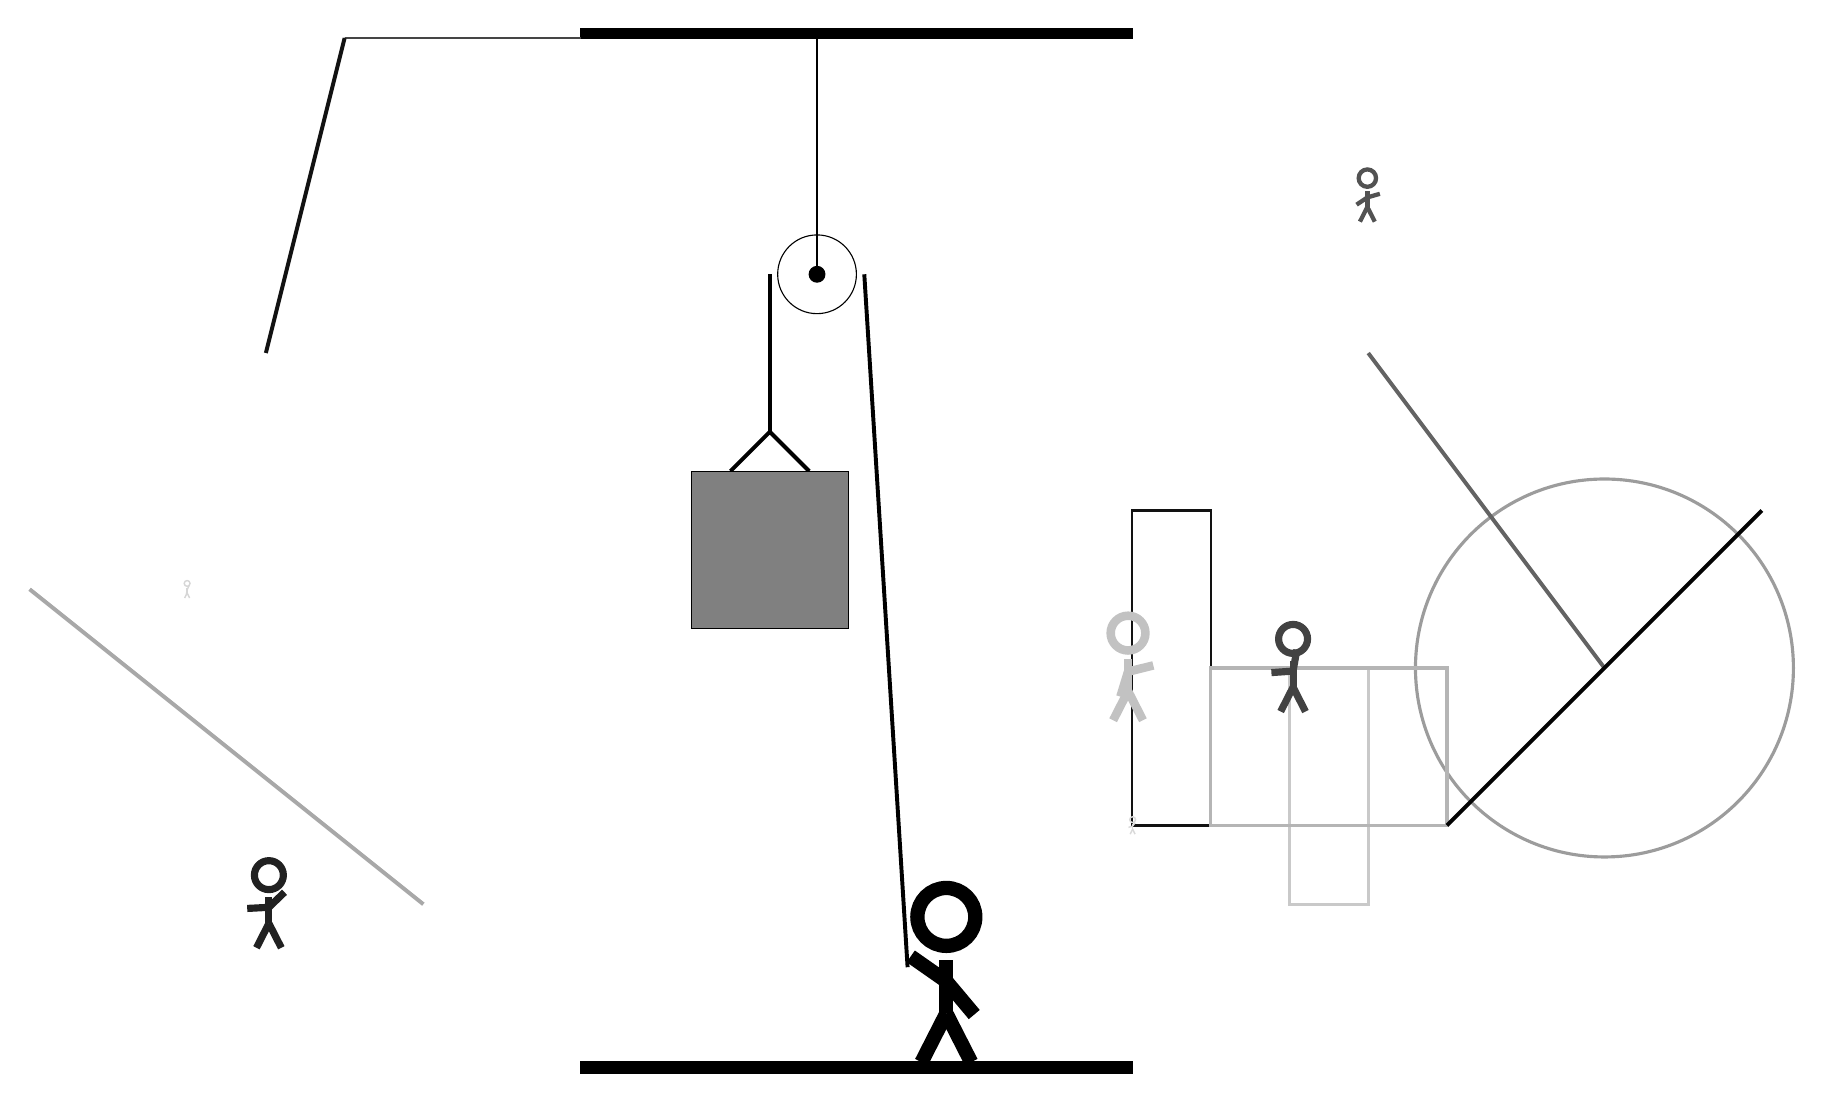
\begin{tikzpicture}
		%%%%% START %%%%%
		
		\draw[fill=black] (-2, 10) rectangle (5, 10.125);
		
		\draw (1, 7) circle (0.5);
		\draw[fill=black] (1, 7) circle (0.1);
		\draw (1, 10) -- (1, 7);
		
		\draw[line width=0.5mm] (-0.1, 4.5) -- (0.4, 5.0) -- (0.9, 4.5);
		\draw[fill=black!50] (-0.6, 4.5) rectangle (1.4, 2.5);
		
		\draw[line width=0.3mm, color=black!93] (5, 0) rectangle (6, 4);
		
		\draw [line width=0.4mm, color=black!39](11, 2) circle (2.4);
		\draw[line width=0.2mm, color=black!73] (-2, 10) rectangle (-5, 10);
		\node[line width=0.7mm, color=black!68] at (8, 8) {\Strichmaxerl[3][34][16]};
		\draw[line width=0.4mm, color=black!21] (7, 2) rectangle (8, -1);
		\draw[line width=0.5mm, color=black!61](8, 6) -- (11, 2);
		
		\draw[line width=0.4mm, color=black!29] (6, 0) rectangle (9, 2);
		\node[line width=0.6mm, color=black!16] at (-7, 3) {\Strichmaxerl[1][81][66]};
		\node[line width=0.3mm, color=black!24] at (5, 2) {\Strichmaxerl[6][73][14]};
		\node[line width=0.2mm, color=black!74] at (7, 2) {\Strichmaxerl[5][4][80]};
		\draw[line width=0.5mm, color=black!93](-5, 10) -- (-6, 6);
		\draw[line width=0.5mm, color=black!34](-4, -1) -- (-9, 3);
		\draw[line width=0.5mm, color=black!99](9, 0) -- (13, 4);
		
		\node[line width=0.3mm, color=black!87] at (-6, -1) {\Strichmaxerl[5][3][44]};
		\node[line width=0.6mm, color=black!15] at (5, 0) {\Strichmaxerl[1][17][53]};
		
		\draw[line width=0.5mm] (0.4, 7) -- (0.4, 5.0);
		\centerarc[line width=0.5mm](1, 7)(0:180:0.6);
		\draw[line width=0.5mm](1.6, 7) -- (2.15, -1.8);
		
		\node at (2.6, -1.9) {\Strichmaxerl[10][-35][-50]};
		
		\draw[fill=black] (-2, -3) rectangle (5, -3.15);
		
		%%%%% END %%%%%
	\end{tikzpicture}
\end{document}